\documentclass{article}
\usepackage[utf8]{inputenc} %кодировка
\usepackage[T2A]{fontenc}
\usepackage[english,russian]{babel} %русификатор 
\usepackage{mathtools} %библиотека матеши
\usepackage[left=1cm,right=1cm,top=2cm,bottom=2cm,bindingoffset=0cm]{geometry} %изменение отступов на листе
\usepackage{amsmath}
\usepackage{graphicx} %библиотека для графики и картинок
\graphicspath{}
\DeclareGraphicsExtensions{.pdf,.png,.jpg}
\usepackage{subcaption}
\usepackage{pgfplots}
\usepackage{float}
\usepackage{listings}


\lstset{
    numbers=left,            % Нумерация строк слева
    numberstyle=\tiny,       % Размер шрифта для номеров строк
    stepnumber=1,            % Нумеровать каждую строку
    numbersep=5pt,           % Расстояние между номерами и кодом
    backgroundcolor=\color{white},  % Цвет фона
    showspaces=false,        % Не показывать пробелы
    showstringspaces=false,  % Не показывать пробелы в строках
    showtabs=false,          % Не показывать табуляцию
    frame=single,            % Рамка вокруг кода
    tabsize=2,               % Размер табуляции
    breaklines=true,         % Автоматический перенос строк
    breakatwhitespace=true   % Переносить строки только по пробелам
}


\begin{document}
% НАЧАЛО ТИТУЛЬНОГО ЛИСТА
\begin{center}
    \Large
    Федеральное государственное автономное \\
    образовательное учреждение высшего образования \\ 
    «Научно-образовательная корпорация ИТМО»\\
    \vspace{0.5cm}
    \large
    Факультет программной инженерии и компьютерной техники \\
    Направление подготовки 09.03.04 Программная инженерия \\
    \vspace{1cm}
    \Large
    \textbf{Отчёт по лабораторной работе №3} \\
        По дисциплине «Распределённые системы хранения данных» ( семестр 6)\\
    \large
    \vspace{8cm}

    \begin{minipage}{.33\textwidth}
    \end{minipage}
    \hfill
    \begin{minipage}{.4\textwidth}
    
        \textbf{Студент}: \vspace{.1cm} \\
        \ Дениченко Александр P3312\\
        \textbf{Практик}:  \\
        \ Осипов Святослав
    \end{minipage}
    \vfill
Санкт-Петербург\\ 2025 г.
\end{center}
\pagestyle{empty}
% КОНЕЦ ТИТУЛЬНОГО ЛИСТА 
\newpage
\pagestyle{plain}

\section*{Задание}
Цель работы - настроить процедуру периодического резервного копирования базы данных, сконфигурированной в ходе выполнения лабораторной работы №2, а также разработать и отладить сценарии восстановления в случае сбоев.

Узел из предыдущей лабораторной работы используется в качестве основного. Новый узел используется в качестве резервного. Учётные данные для подключения к новому узлу выдаёт преподаватель. В сценариях восстановления необходимо использовать копию данных, полученную на первом этапе данной лабораторной работы.

\section*{Этап 1. Резервное копирование}
Настроить резервное копирование с основного узла на резервный следующим образом:
Периодические полные копии с помощью SQL Dump.
По расписанию (cron) раз в сутки, методом SQL Dump с сжатием. Созданные архивы должны сразу перемещаться на резервный хост, они не должны храниться на основной системе. Срок хранения архивов на резервной системе - 4 недели. По истечении срока хранения, старые архивы должны автоматически уничтожаться.
\\ \\
Изначально сделаем донастройку конфигураций прежней базы данных.
\begin{lstlisting}[caption={kitty}, label={lst:example}]
    docker create --name postgres-cont-1 -e POSTGRES_PASSWORD=root -p 9193:9193 postgres
\end{lstlisting}

\begin{lstlisting}[caption={kitty}, label={lst:example}]
    docker start postgres-cont-1 
    docker exec -it postgres-cont-1 /bin/bash
\end{lstlisting}

Изменение некоторых настроек разрешений
\begin{lstlisting}[caption={postgresql.conf}, label={lst:example}]
    listen_addresses = '*'
\end{lstlisting}
\begin{lstlisting}[caption={pg\_hba.conf}, label={lst:example}]
    host    all    all    0.0.0.0/0    scram-sha-256
\end{lstlisting}
Подключение к первому узлу теперь выглядит следующим образом.
\begin{lstlisting}[caption={kitty}, label={lst:example}]
    psql -h 127.0.0.1 -p 9193 -U postgres -d postgres 
    psql -h 127.0.0.1 -p 9193 -U postgres -d fatrednews     
    psql -h 127.0.0.1 -p 9193 -U fatreduser -d fatrednews 
\end{lstlisting}

\textbf{postgres - root}

\textbf{fatreduser - changeMe}
\\ \\
Табличные пространства из прошлой лабы

\begin{lstlisting}[caption={kitty}, label={lst:example}]
    List of tablespaces
    Name    |  Owner   |         Location          | Access privileges | Options |  Size   | Description 
    ------------+----------+---------------------------+-------------------+---------+---------+-------------
    pg_default | postgres |                           |                   |         | 22 MB   | 
    pg_global  | postgres |                           |                   |         | 565 kB  | 
    sgk31      | postgres | /var/lib/postgresql/sgk31 |                   |         | 0 bytes | 
    yrp30      | postgres | /var/lib/postgresql/yrp30 |                   |         | 0 bytes | 
    yva58      | postgres | /var/lib/postgresql/yva58 |                   |         | 0 bytes | 
    (5 rows)
\end{lstlisting}


Создан узел для хранения бэкапов

\begin{lstlisting}[caption={kitty}, label={lst:example}]
    docker create --name postgres-backup -p 9194:9193 ubuntu:latest tail -f /dev/null
\end{lstlisting}

Добавлены утилиты на резервном узле и на основном
\begin{lstlisting}[caption={kitty}, label={lst:example}]
    apt-get install -y cron openssh-client openssh-server gzip
\end{lstlisting}

Была сделана сеть докер для обмена

\begin{lstlisting}[caption={kitty}, label={lst:example}]
    docker network create --driver bridge postgres-backup-net 
    docker network connect postgres-backup-net postgres-cont-1 postgres-backup
    docker restart postgres-cont-1 postgres-backup
\end{lstlisting}

Добавим конфиг в сервер 
\begin{lstlisting}[caption={kitty}, label={lst:example}]
    echo "PermitRootLogin yes" >> /etc/ssh/sshd_config
    chmod 700 /root/.ssh
    mkdir -p /run/sshd
    chmod 755 /run/sshd
    service ssh start
\end{lstlisting}

Добавлены ключи для упрощения обмена данными на основном сервере
\begin{lstlisting}[caption={kitty}, label={lst:example}]
    ssh-keygen -t rsa -b 4096
    cat ~/.ssh/id_rsa.pub 
\end{lstlisting}

И добавили ключи в резервный узел
\begin{lstlisting}[caption={kitty}, label={lst:example}]
    vim ~/.ssh/authorized_keys ....
\end{lstlisting}

Настройка скрипта для копирования
\begin{lstlisting}[caption={kitty}, label={lst:example}]
#!/bin/bash

PG_USER="postgres"
BACKUP_DIR="/tmp/backups"
REMOTE_HOST="help"
REMOTE_DIR="/backups"
TIMESTAMP=$(date +%Y%m%d_%H%M%S)
FULL_BACKUP_FILE="full_backup-$TIMESTAMP.sql.gz"
TABLESPACE_INFO_FILE="tablespace_info-$TIMESTAMP.txt"
LOG_FILE="/tmp/backup_log.txt"

echo "Starting backup: $TIMESTAMP" >> $LOG_FILE
mkdir -p $BACKUP_DIR

echo "Creating database dump..." >> $LOG_FILE
if pg_dumpall -p 9193 -U $PG_USER | gzip > $BACKUP_DIR/$FULL_BACKUP_FILE; then
    echo "Backup created successfully: $FULL_BACKUP_FILE" >> $LOG_FILE
else
    echo "Backup failed" >> $LOG_FILE
    exit 1
fi

echo "Collecting tablespace information..." >> $LOG_FILE
psql -p 9193 -U $PG_USER -c "SELECT spcname, pg_catalog.pg_tablespace_location(oid) FROM pg_catalog.pg_tablespace;" > $BACKUP_DIR/$TABLESPACE_INFO_FILE
echo "Tablespace information collected" >> $LOG_FILE

echo "Transferring files to backup server..." >> $LOG_FILE
if scp $BACKUP_DIR/$FULL_BACKUP_FILE $BACKUP_DIR/$TABLESPACE_INFO_FILE $REMOTE_HOST:$REMOTE_DIR/; then
    echo "Backup transferred successfully" >> $LOG_FILE
else
    echo "Transfer failed" >> $LOG_FILE
    exit 1
fi

rm $BACKUP_DIR/$FULL_BACKUP_FILE $BACKUP_DIR/$TABLESPACE_INFO_FILE

echo "Backup script completed" >> $LOG_FILE  
\end{lstlisting}

Сама настройка для автоматизации на основном хосте
\begin{lstlisting}[caption={kitty}, label={lst:example}]
    crontab -e 
    */1 * * * * /backup.sh
    cron
\end{lstlisting}

Настройка для автоматизации на доп хосте
\begin{lstlisting}[caption={kitty}, label={lst:example}]
    crontab -e 
    */2 * * * * /cleanup_dumps.sh
    cron
\end{lstlisting}

\section*{Расчет объема резервных копий через месяц}

Исходные данные:

- Средний объем новых данных в БД за сутки: 950 МБ.

- Средний объем измененных данных за сутки: 150 МБ.

- Период хранения резервных копий: 4 недели (28 дней).
\\
Предположения:

1. Бэкап делается полностью (включает все данные, а не только новые или измененные).

2. Измененные данные не увеличивают общий объем бэкапа, так как они уже входят в полную копию.

3. Объем БД увеличивается со временем за счет новых данных.
\\
Каждый день создается новая полная резервная копия.  
Объем бэкапа на n-й день равен всему объему базы данных на тот момент.

Объем базы через n дней можно выразить как:

\[
V(n) = V_0 + 950 \times n
\]

Где:

- \( V_0 \) — начальный объем базы (пусть 0 для расчета за 1 месяц),

- 950 — рост базы в день.
\\ \\
Общий объем всех бэкапов за 28 дней:
\[
V_{\text{total}} = \sum_{n=1}^{28} (950 \times n)
\]

---

Рассчитаем сумму:

\[
V_{\text{total}} = 950 \times (1 + 2 + ... + 28)
\]

Сумма арифметической прогрессии:
\[
S = \frac{n (n+1)}{2}
\]
Где \( n = 28 \):

\[
S = \frac{28 \times 29}{2} = 406
\]

Подставляем:
\[
V_{\text{total}} = 950 \times 406 = 385 700 \text{ МБ} = 385.7 \text{ ГБ}
\]

\section*{Потеря основного узла}

\begin{lstlisting}[caption={kitty}, label={lst:example}]
#!/bin/bash

set -e  

PGDATA=${PGDATA:-"/var/lib/postgresql/data"}
BACKUP_DIR="/backups"
PORT=9193
TBSP_BASE="/var/lib/postgresql"  

TABLESPACES=("yva58" "yrp30" "sgk31")

if ! command -v pg_ctl &> /dev/null; then
    PG_PATHS=(
        "/usr/lib/postgresql/17/bin"
        "/usr/lib/postgresql/*/bin"
        "/usr/pgsql-17/bin"
        "/usr/pgsql-*/bin"
        "/opt/postgresql/17/bin"
        "/opt/postgresql/*/bin"
    )
    
    for pg_path in "${PG_PATHS[@]}"; do
        for possible_path in $pg_path; do
            if [ -d "$possible_path" ] && [ -x "$possible_path/pg_ctl" ]; then
                export PATH="$possible_path:$PATH"
                break 2
            fi
        done
    done
    
    if ! command -v pg_ctl &> /dev/null; then
        exit 1
    fi
fi

LATEST_BACKUP=$(ls -t ${BACKUP_DIR}/full_backup-*.sql.gz 2>/dev/null | head -1)
if [ -z "$LATEST_BACKUP" ]; then
    exit 1
fi


AVAILABLE_LOCALES=$(locale -a)
if echo "$AVAILABLE_LOCALES" | grep -q "en_US.utf8"; then
    REPLACEMENT_LOCALE="en_US.utf8"
elif echo "$AVAILABLE_LOCALES" | grep -q "en_US.UTF-8"; then
    REPLACEMENT_LOCALE="en_US.UTF-8"
elif echo "$AVAILABLE_LOCALES" | grep -q "C.UTF-8"; then
    REPLACEMENT_LOCALE="C.UTF-8"
else
    REPLACEMENT_LOCALE="C"
fi

TEMP_DUMP=$(mktemp)

gunzip -c "$LATEST_BACKUP" | sed \
    -e "s/LOCALE = 'en_US.utf8'/LOCALE = '$REPLACEMENT_LOCALE'/g" \
    -e "s/LOCALE = 'ru_RU.utf8'/LOCALE = '$REPLACEMENT_LOCALE'/g" \
    -e "s/LOCALE = 'en_US.UTF-8'/LOCALE = '$REPLACEMENT_LOCALE'/g" \
    -e "s/LOCALE = 'ru_RU.UTF-8'/LOCALE = '$REPLACEMENT_LOCALE'/g" \
    > "$TEMP_DUMP"

for tbsp in "${TABLESPACES[@]}"; do
    tbsp_dir="$TBSP_BASE/$tbsp"
    mkdir -p "$tbsp_dir"
    chown -R postgres:postgres "$tbsp_dir"
    chmod 700 "$tbsp_dir"
done

if pg_ctl -D "$PGDATA" status > /dev/null 2>&1; then
    pg_ctl -D "$PGDATA" stop -m fast
fi

if [ -d "$PGDATA" ]; then
    rm -rf "${PGDATA:?}"/* 
fi

if ! command -v initdb &> /dev/null; then
    exit 1
fi

initdb -D "$PGDATA" --locale="$REPLACEMENT_LOCALE" || {
    exit 1
}

echo "port = $PORT" >> "$PGDATA/postgresql.conf"
echo "listen_addresses = '*'" >> "$PGDATA/postgresql.conf"
echo "host all all all md5" >> "$PGDATA/pg_hba.conf"


pg_ctl -D "$PGDATA" -o "-p $PORT" start || {
    if [ -f "$PGDATA/log/postgresql.log" ]; then
        tail "$PGDATA/log/postgresql.log"
    elif [ -d "$PGDATA/log" ]; then
        find "$PGDATA/log" -type f -name "*.log" | xargs tail
    fi
    exit 1
}

if ! pg_ctl -D "$PGDATA" status > /dev/null 2>&1; then
    exit 1
fi

cat "$TEMP_DUMP" | psql -p $PORT -U postgres postgres

if ! psql -p $PORT -U postgres -lqt | cut -d \| -f 1 | grep -qw fatrednews; then
    psql -p $PORT -U postgres -c "CREATE DATABASE fatrednews WITH TEMPLATE = template0 ENCODING = 'UTF8' LOCALE_PROVIDER = libc LOCALE = '$REPLACEMENT_LOCALE';"
    psql -p $PORT -U postgres -c "ALTER DATABASE fatrednews OWNER TO postgres;"
fi

rm -f "$TEMP_DUMP"

sleep 5

pg_ctl -D "$PGDATA" restart || {
    exit 1
}

psql -p $PORT -U postgres -c "\l"
\end{lstlisting}


Пример восстановления базы данных
\\ \\
Запуск резервного узла
\begin{lstlisting}[caption={kitty}, label={lst:example}]
    docker exec -it postgres-backup /bin/bash
\end{lstlisting}

Должно быть включено ssh и общая есть у двух контейнеров.
\begin{lstlisting}[caption={kitty}, label={lst:example}]
    service ssh start
\end{lstlisting}

Делаем типо последний бэкап с основного узла перед его выходом из строя
\begin{lstlisting}[caption={kitty}, label={lst:example}]
root@44dfe2ea5829:/# ./backup.sh 
    full_backup-20250403_162858.sql.gz                      100% 1699    10.1MB/s   00:00    
    tablespace_info-20250403_162858.txt                     100%  242     3.0MB/s   00:00 
\end{lstlisting}

Восстанавливаем кластер на резервном узле
\begin{lstlisting}[caption={kitty}, label={lst:example}]
    root@49f86d293fa3:/# sudo -u postgres bash /restore.sh 
\end{lstlisting}

\section*{Повреждение файлов БД}
По факту мы можем применять скрипт для основного узля в любом состоянии бд, так как резервная копия находится на резервном узле, просто происходит запрос в скрипте и развёртывание нового кластера в новой директории

\begin{lstlisting}[caption={kitty}, label={lst:example}]
    root@44dfe2ea5829:/# ./restore.sh 
\end{lstlisting}

Сам скрипт
\begin{lstlisting}[caption={kitty}, label={lst:example}]
#!/bin/bash


PG_USER="postgres"
REMOTE_HOST="help"
REMOTE_BACKUP_DIR="/backups"
LOCAL_TEMP_DIR="/tmp/restore"
NEW_PGDATA="/var/lib/postgresql/new_data"  
PORT=9193
LOG_FILE="/tmp/restore_log.txt"
POSTGRES_CONF="/etc/postgresql/15/main/postgresql.conf" 

TABLESPACES=("yva58" "yrp30" "sgk31")
TBSP_BASE="/var/lib/postgresql"


mkdir -p $LOCAL_TEMP_DIR

LATEST_BACKUP=$(ssh $REMOTE_HOST "ls -t $REMOTE_BACKUP_DIR/full_backup-*.sql.gz | head -1")
LATEST_TABLESPACE_INFO=$(ssh $REMOTE_HOST "ls -t $REMOTE_BACKUP_DIR/tablespace_info-*.txt | head -1")

if [ -z "$LATEST_BACKUP" ]; then
    exit 1
fi

BACKUP_FILENAME=$(basename "$LATEST_BACKUP")
TABLESPACE_FILENAME=$(basename "$LATEST_TABLESPACE_INFO")


scp "$REMOTE_HOST:$LATEST_BACKUP" "$LOCAL_TEMP_DIR/$BACKUP_FILENAME"
scp "$REMOTE_HOST:$LATEST_TABLESPACE_INFO" "$LOCAL_TEMP_DIR/$TABLESPACE_FILENAME"

systemctl stop postgresql || {
    su - postgres -c "pg_ctl stop -D /var/lib/postgresql/15/main -m fast"
}

mkdir -p $NEW_PGDATA
chown postgres:postgres $NEW_PGDATA
chmod 700 $NEW_PGDATA

for tbsp in "${TABLESPACES[@]}"; do
    tbsp_dir="$TBSP_BASE/$tbsp"
    mkdir -p "$tbsp_dir"
    chown postgres:postgres "$tbsp_dir"
    chmod 700 "$tbsp_dir"
done

AVAILABLE_LOCALES=$(locale -a)
if echo "$AVAILABLE_LOCALES" | grep -q "en_US.utf8"; then
    LOCALE="en_US.utf8"
elif echo "$AVAILABLE_LOCALES" | grep -q "en_US.UTF-8"; then
    LOCALE="en_US.UTF-8"
elif echo "$AVAILABLE_LOCALES" | grep -q "C.UTF-8"; then
    LOCALE="C.UTF-8"
else
    LOCALE="C"
fi

TEMP_DUMP=$(mktemp)

gunzip -c "$LOCAL_TEMP_DIR/$BACKUP_FILENAME" | sed \
    -e "s/LOCALE = 'en_US.utf8'/LOCALE = '$LOCALE'/g" \
    -e "s/LOCALE = 'ru_RU.utf8'/LOCALE = '$LOCALE'/g" \
    -e "s/LOCALE = 'en_US.UTF-8'/LOCALE = '$LOCALE'/g" \
    -e "s/LOCALE = 'ru_RU.UTF-8'/LOCALE = '$LOCALE'/g" \
    > "$TEMP_DUMP"

su - postgres -c "initdb -D $NEW_PGDATA --locale=$LOCALE" || {
    exit 1
}


sed -i "s|data_directory = '.*'|data_directory = '$NEW_PGDATA'|" $POSTGRES_CONF

systemctl start postgresql || {
    su - postgres -c "pg_ctl start -D $NEW_PGDATA -o '-p $PORT'" || {
        exit 1
    }
}

su - postgres -c "cat $TEMP_DUMP | psql -p $PORT"

if ! su - postgres -c "psql -p $PORT -lqt" | cut -d \| -f 1 | grep -qw fatrednews; then
    su - postgres -c "psql -p $PORT -c \"CREATE DATABASE fatrednews WITH TEMPLATE = template0 ENCODING = 'UTF8' LOCALE_PROVIDER = libc LOCALE = '$LOCALE';\""
    su - postgres -c "psql -p $PORT -c \"ALTER DATABASE fatrednews OWNER TO postgres;\""
fi

rm -f "$TEMP_DUMP"

systemctl restart postgresql || {
    su - postgres -c "pg_ctl restart -D $NEW_PGDATA -o '-p $PORT'" || {
        exit 1
    }
}

if systemctl is-active postgresql >/dev/null; then
else
    if su - postgres -c "pg_ctl status -D $NEW_PGDATA" >/dev/null; then
    else
        exit 1
    fi
fi

su - postgres -c "psql -p $PORT -c '\l'" | tee -a $LOG_FILE

\end{lstlisting}

\section*{Логическое повреждение данных}

1. Подготовка среды для архивирования WAL

Сначала я создал директорию для хранения WAL архивов:

\begin{lstlisting}[caption={kitty}, label={lst:example}]
    mkdir -p /var/lib/postgresql/wal_archive
    chown postgres:postgres /var/lib/postgresql/wal_archive
\end{lstlisting}


Затем настроил параметры WAL архивирования в PostgreSQL:

\begin{lstlisting}[caption={kitty}, label={lst:example}]
su - postgres -c "psql -p 9193 -c \"ALTER SYSTEM SET wal_level = 'replica';\""
su - postgres -c "psql -p 9193 -c \"ALTER SYSTEM SET archive_mode = 'on';\""
su - postgres -c "psql -p 9193 -c \"ALTER SYSTEM SET archive_command = 'cp %p /var/lib/postgresql/wal_archive/%f';\""
\end{lstlisting}


После этого перезапустил PostgreSQL для применения настроек:
\begin{lstlisting}[caption={kitty}, label={lst:example}]
    su - postgres -c "pg_ctl restart -D /var/lib/postgresql/data -o '-p 9193'"
\end{lstlisting}


2. Создание базовой резервной копии
\\
Создал директорию для хранения базовой резервной копии:

\begin{lstlisting}[caption={kitty}, label={lst:example}]
    mkdir -p /tmp/pg_basebackup
    chown postgres:postgres /tmp/pg_basebackup
\end{lstlisting}

Выполнил базовое резервное копирование:

\begin{lstlisting}[caption={kitty}, label={lst:example}]
    su - postgres -c "pg_basebackup -D /tmp/pg_basebackup -p 9193 -X stream -c fast -P"
\end{lstlisting}

3. Добавление тестовых данных
\\
Создал тестовые таблицы для демонстрации:

\begin{lstlisting}[caption={kitty}, label={lst:example}]
    su - postgres -c "psql -p 9193 -c \"
    CREATE TABLE IF NOT EXISTS test_parent (
        id SERIAL PRIMARY KEY,
        name VARCHAR(100),
        created_at TIMESTAMP DEFAULT CURRENT_TIMESTAMP
    );
    
    CREATE TABLE IF NOT EXISTS test_child (
        id SERIAL PRIMARY KEY,
        parent_id INTEGER REFERENCES test_parent(id),
        description TEXT,
        created_at TIMESTAMP DEFAULT CURRENT_TIMESTAMP
    );\""
    su - postgres -c "psql -p 9193 -c \"
    INSERT INTO test_parent (name) VALUES 
        ('Parent 1'),
        ('Parent 2'),
        ('Parent 3');
        
    INSERT INTO test_child (parent_id, description) VALUES 
        (1, 'Child of Parent 1'),
        (2, 'Child of Parent 2'),
        (3, 'Child of Parent 3');\""
\end{lstlisting}




Зафиксировал время перед добавлением новых данных:
\begin{lstlisting}[caption={kitty}, label={lst:example}]
    BEFORE_INSERT_TIME="2025-04-03 21:30:15"
\end{lstlisting}

Добавил новые записи в таблицы:
\begin{lstlisting}[caption={kitty}, label={lst:example}]
    su - postgres -c "psql -p 9193 -c \"
    INSERT INTO test_parent (name) VALUES 
        ('New Parent 1'),
        ('New Parent 2'),
        ('New Parent 3');
        
    INSERT INTO test_child (parent_id, description) VALUES 
        (4, 'Child of New Parent 1'),
        (5, 'Child of New Parent 2'),
        (6, 'Child of New Parent 3');\""\
\end{lstlisting}

Переключил WAL для обеспечения архивирования:
\begin{lstlisting}[caption={kitty}, label={lst:example}]
    su - postgres -c "psql -p 9193 -c \"SELECT pg_switch_wal();\""
\end{lstlisting}

4. Симуляция логического повреждения данных
\\
Зафиксировал время перед внесением ошибки:
\begin{lstlisting}[caption={kitty}, label={lst:example}]
    ERROR_TIME="2025-04-03 21:35:25"
\end{lstlisting}

Посмотрел текущие данные и выполнил некорректное обновление внешних ключей:

\begin{lstlisting}[caption={kitty}, label={lst:example}]
    su - postgres -c "psql -p 9193 -c \"
    UPDATE test_child
    SET parent_id = (
        SELECT ceil(random() * 1000)::int
    )
    WHERE parent_id IS NOT NULL;

    SELECT * FROM test_child LIMIT 10;\""
\end{lstlisting}




После этого снова переключил WAL для архивирования:
\begin{lstlisting}[caption={kitty}, label={lst:example}]
    su - postgres -c "psql -p 9193 -c \"SELECT pg_switch_wal();\""
\end{lstlisting}

5. Восстановление данных до момента перед ошибкой

Остановил PostgreSQL:
\begin{lstlisting}[caption={kitty}, label={lst:example}]
    su - postgres -c "pg_ctl stop -D /var/lib/postgresql/data -m fast"
\end{lstlisting}

Скопировал базовую резервную копию в директорию данных:
\begin{lstlisting}[caption={kitty}, label={lst:example}]
    rm -rf /var/lib/postgresql/data/*
    cp -a /tmp/pg_basebackup/* /var/lib/postgresql/data/
    chown -R postgres:postgres /var/lib/postgresql/data
\end{lstlisting}

```

Настроил конфигурацию восстановления для PostgreSQL 17:
\begin{lstlisting}[caption={kitty}, label={lst:example}]
    cat > /var/lib/postgresql/data/postgresql.conf << EOF

\end{lstlisting}
Параметры восстановления
\begin{lstlisting}[caption={kitty}, label={lst:example}]
    restore_command = 'cp /var/lib/postgresql/wal_archive/%f %p'
    recovery_target_time = '2025-04-03 21:35:25'
    recovery_target_action = 'pause'
    EOF

    touch /var/lib/postgresql/data/recovery.signal
    chown postgres:postgres /var/lib/postgresql/data/recovery.signal
\end{lstlisting}


Запустил PostgreSQL в режиме восстановления:
\begin{lstlisting}[caption={kitty}, label={lst:example}]
    su - postgres -c "pg_ctl start -D /var/lib/postgresql/data -o '-p 9193'"
\end{lstlisting}
Проверил статус восстановления и продолжил восстановление:
\begin{lstlisting}[caption={kitty}, label={lst:example}]
    su - postgres -c "psql -p 9193 -c \"SELECT pg_is_in_recovery();\""
    su - postgres -c "psql -p 9193 -c \"SELECT pg_wal_replay_resume();\""
\end{lstlisting}


После завершения восстановления удалил recovery.signal и перезапустил PostgreSQL в обычном режиме:
\begin{lstlisting}[caption={kitty}, label={lst:example}]
    rm -f /var/lib/postgresql/data/recovery.signal
    su - postgres -c "pg_ctl restart -D /var/lib/postgresql/data -o '-p 9193'"  
\end{lstlisting}


6. Проверка результатов восстановления

Проверил данные в таблице после восстановления:
\begin{lstlisting}[caption={kitty}, label={lst:example}]
    su - postgres -c "psql -p 9193 -c \"SELECT * FROM test_child LIMIT 10;\""
\end{lstlisting}


\end{document}



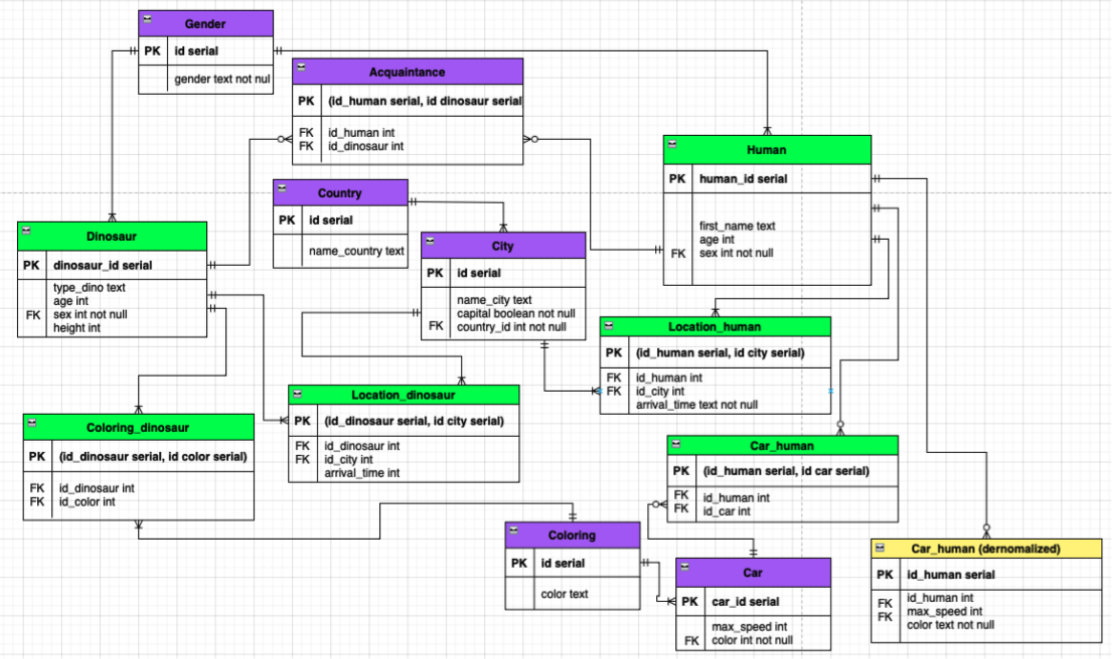
\includegraphics[width=.9\textwidth]{123}

\begin{lstlisting}[caption={kitty}, label={lst:example}]

\end{lstlisting}